\section{Relaxation due to noise}
% A system coupled to resonators in thermal equilibrium energy exchange
% depends   on    the   temperature   of   these    resonators.    When
% $ kT>>\hbar\omega $ photons will  be exchanged between the medium and
% system. When $ kT<<\hbar\omega $  the system will remain indefinitely
% in the ground state
\subsection{Relaxation from the noise spectrum}

\begin{figure}[h]
  \centering 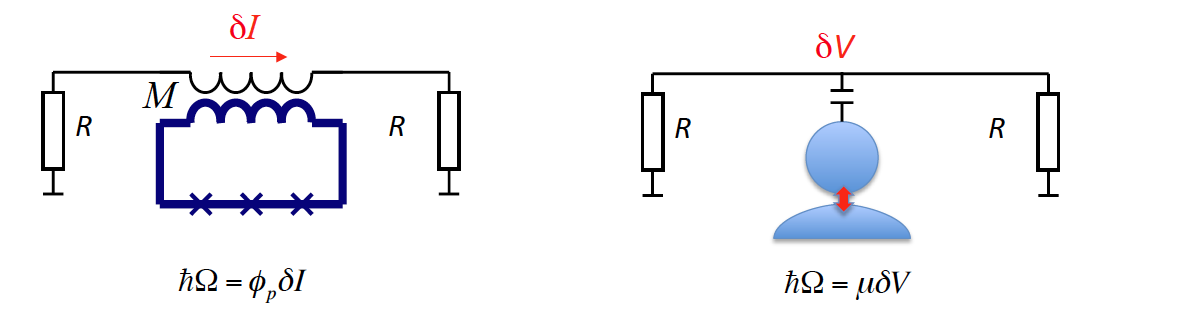
\includegraphics[height=4cm]{noise1}
\end{figure}

\noindent

\noindent In the  systems above noise may come from  current or voltage
fluctuations. We  shall analyse the  latter case, in which  the voltage
fluctuation acts as an effective driving field

\begin{equation}\label{noise1}
  \mathcal{H} = -\frac{\hbar\omega}{2}\sigma_z+\frac{\mu\delta V(\omega)}{2}\sigma_x\cos(\omega t);\quad\delta V(\omega) = \frac{1}{T}\int_{-T/2}^{T/2}\delta V(t e^{-i\omega t})dt,
\end{equation}

\noindent and after applying the RWA

\begin{equation}\label{noise2}
  \mathcal{H} = \frac{\mu\delta V(\omega)}{2}\sigma_x,
\end{equation}

\noindent the evolution of a system state

\begin{equation}\label{noise3}
  U(T)\iket{0} = \iket{0} - \frac{\mu\delta V(\omega)}{2}\frac{T}{\hbar}\iket{1} \quad \rightarrow \quad P_1 = \frac{\mu^2T^2}{4\hbar^2}\iaverage{\delta V^2},
\end{equation}

\noindent and incorporating  the spectral noise density $  S(\Omega) $ which
we integrate  over in  the frequency  range $  \Delta\omega =  2\pi/T $
(longer  acquisition time  means narrower  spectrum of  noise since  we
average more  and more, and only  low frequency remains will  remain in
the system.)

\begin{equation}\label{noise4}
  \begin{aligned}
    \iaverage{\delta V^2}&=S(\omega)\frac{2\pi}{T}\\
    P_1 &= \frac{\mu^2T^2}{4\hbar^2}\iaverage{\delta V^2}
  \end{aligned}\Rightarrow P_1 = \frac{\pi\mu^2}{2\hbar^2}S(\omega)T \rightarrow \text{ rate of
    excitation } \approx \Gamma = \frac{\pi\mu^2}{2\hbar^2}S(\omega).
\end{equation}


\begin{figure}[h]
  \centering 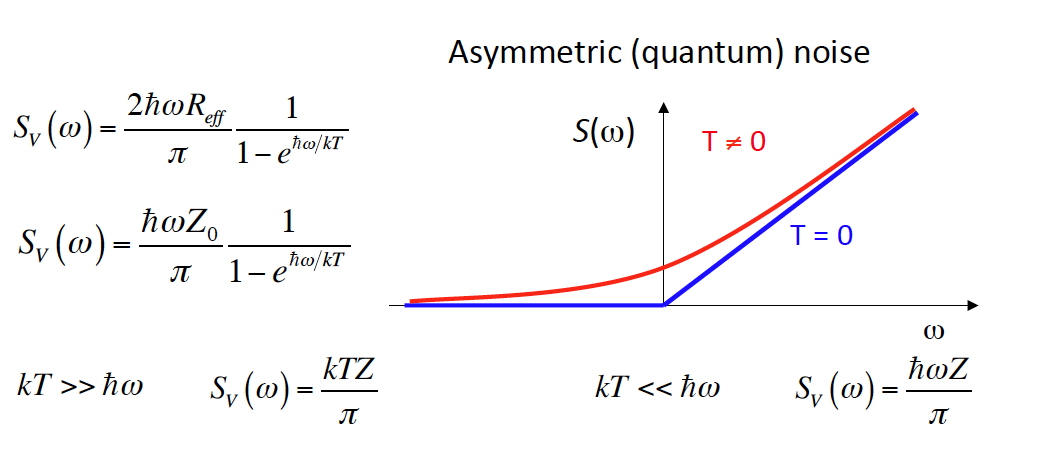
\includegraphics[height=4cm]{noise2}
\end{figure}

\newpage
